
\begin{figure}
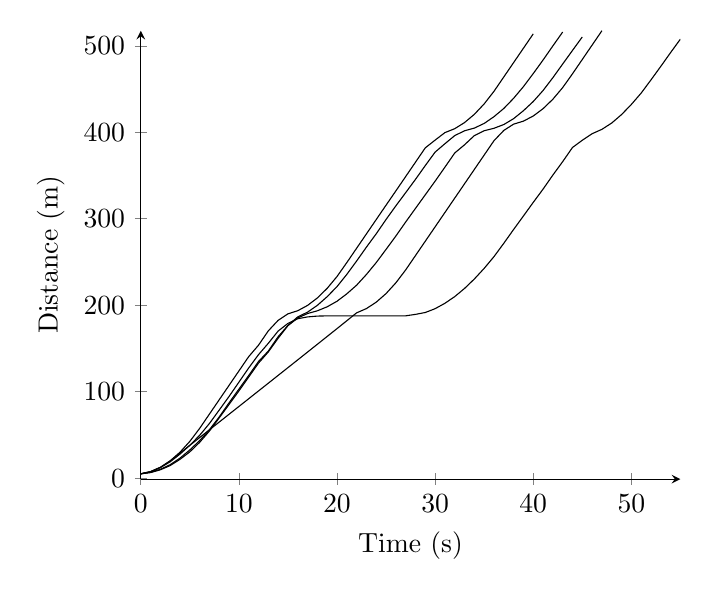
\begin{tikzpicture}
\begin{axis}[
legend style={
	anchor=west
},
axis x line=bottom,
axis y line=left,
ymin=-1,
point meta=explicit symbolic,
xlabel=Time (s),
ylabel=Distance (m)
]
\addplot[] coordinates {
(0, 5.1)
(1, 7.50746572556)
(2, 12.3019236314)
(3, 18.972925778)
(4, 27.9059489134)
(5, 38.093907686)
(6, 49.5696963296)
(7, 63.3091187951)
(8, 78.867049009)
(9, 94.5878329703)
(10, 111.024317915)
(11, 127.500875795)
(12, 142.879206964)
(13, 156.032998112)
(14, 170.169046938)
(15, 179.027686887)
(16, 184.399973394)
(17, 186.530360973)
(18, 187.478707481)
(19, 187.730761234)
(20, 187.773324537)
(21, 187.773324537)
(22, 187.773324537)
(23, 187.773324537)
(24, 187.773324537)
(25, 187.773324537)
(26, 187.773324537)
(27, 187.773324537)
(28, 189.463801494)
(29, 191.628877469)
(30, 196.020459831)
(31, 202.29337637)
(32, 210.000388873)
(33, 219.447877933)
(34, 230.383076814)
(35, 242.645688463)
(36, 256.234973966)
(37, 271.649158066)
(38, 287.617778644)
(39, 303.213341855)
(40, 318.936771185)
(41, 334.248543897)
(42, 350.518991016)
(43, 366.054213301)
(44, 382.414404809)
(45, 390.791606815)
(46, 398.351017723)
(47, 403.40891413)
(48, 410.7187545)
(49, 420.472956825)
(50, 432.198137953)
(51, 445.334396523)
(52, 460.5727204)
(53, 476.209282838)
(54, 492.168776512)
(55, 507.752232795)
};
\addplot[] coordinates {
(0, 5.1)
(1, 7.6)
(2, 12.6)
(3, 20.1)
(4, 29.0740249671)
(5, 38.0486569992)
(6, 47.0239943627)
(7, 56.0001577571)
(8, 64.9772971093)
(9, 73.9556009985)
(10, 82.9353099838)
(11, 91.9167358612)
(12, 100.900290181)
(13, 109.886527676)
(14, 118.876214602)
(15, 127.870440439)
(16, 136.870808998)
(17, 145.879783896)
(18, 154.90126101)
(19, 163.932926934)
(20, 172.988205725)
(21, 182.087972691)
(22, 191.224165334)
(23, 196.154399366)
(24, 203.584633398)
(25, 213.51486743)
(26, 225.945101462)
(27, 240.875335494)
(28, 257.475335494)
(29, 274.075335494)
(30, 290.675335494)
(31, 307.275335494)
(32, 323.875335494)
(33, 340.475335494)
(34, 357.075335494)
(35, 373.675335494)
(36, 390.275335494)
(37, 402.139712731)
(38, 409.434954257)
(39, 412.880617226)
(40, 418.826280194)
(41, 427.271943163)
(42, 438.217606131)
(43, 451.6632691)
(44, 467.608932069)
(45, 484.208932069)
(46, 500.808932069)
(47, 517.408932069)
};
\addplot[] coordinates {
(0, 5.1)
(1, 6.48752680679)
(2, 9.73681294728)
(3, 14.6608508145)
(4, 21.8077667566)
(5, 30.473428991)
(6, 41.455300459)
(7, 54.6064227551)
(8, 69.8611392531)
(9, 85.3298044756)
(10, 100.892814729)
(11, 116.974943968)
(12, 133.09811184)
(13, 146.048069123)
(14, 161.839393635)
(15, 176.414756614)
(16, 185.28594519)
(17, 190.431897105)
(18, 193.588637962)
(19, 198.224208699)
(20, 204.62531294)
(21, 213.216488869)
(22, 223.200198343)
(23, 235.613722109)
(24, 249.373938059)
(25, 264.589455232)
(26, 280.032983421)
(27, 296.25009529)
(28, 312.024160223)
(29, 327.756589207)
(30, 343.478534729)
(31, 359.666631523)
(32, 376.073554074)
(33, 385.559733408)
(34, 396.200842335)
(35, 401.81553945)
(36, 404.647200893)
(37, 408.965038555)
(38, 415.740496458)
(39, 424.956147837)
(40, 435.540463652)
(41, 448.271291095)
(42, 463.11428527)
(43, 478.917150431)
(44, 494.627972253)
(45, 510.227188176)
};
\addplot[] coordinates {
(0, 5.1)
(1, 6.88294769808)
(2, 10.3482719734)
(3, 15.662766185)
(4, 23.2812326435)
(5, 32.7029330716)
(6, 43.4564170083)
(7, 56.0980914887)
(8, 70.8879514823)
(9, 87.189661168)
(10, 102.972262247)
(11, 118.752811527)
(12, 134.950527415)
(13, 147.021430975)
(14, 163.603287389)
(15, 176.674207415)
(16, 186.577755946)
(17, 192.04110153)
(18, 199.91907466)
(19, 209.919501137)
(20, 221.559289332)
(21, 235.697440711)
(22, 251.159288924)
(23, 267.222073803)
(24, 282.66722806)
(25, 299.17630188)
(26, 314.955045881)
(27, 330.205823153)
(28, 345.577512221)
(29, 361.553660019)
(30, 377.063975996)
(31, 386.792220794)
(32, 396.181205971)
(33, 401.755667255)
(34, 404.86644195)
(35, 410.24108963)
(36, 418.063958801)
(37, 427.540603725)
(38, 439.292918064)
(39, 452.77996707)
(40, 467.868010934)
(41, 483.540233343)
(42, 499.860955328)
(43, 515.905423619)
};
\addplot[] coordinates {
(0, 5.1)
(1, 7.6)
(2, 12.6)
(3, 20.1)
(4, 30.1)
(5, 42.6)
(6, 57.6)
(7, 74.2)
(8, 90.8)
(9, 107.4)
(10, 124.0)
(11, 140.6)
(12, 153.81)
(13, 170.41)
(14, 182.536224097)
(15, 190.065647988)
(16, 193.69332809)
(17, 199.821008192)
(18, 208.448688293)
(19, 219.576368395)
(20, 233.204048497)
(21, 249.331728598)
(22, 265.931728598)
(23, 282.531728598)
(24, 299.131728598)
(25, 315.731728598)
(26, 332.231728598)
(27, 348.831728598)
(28, 365.431728598)
(29, 382.031728598)
(30, 390.95706971)
(31, 399.634779459)
(32, 404.184786402)
(33, 411.234793345)
(34, 420.784800287)
(35, 432.83480723)
(36, 447.384814173)
(37, 463.984814173)
(38, 480.584814173)
(39, 497.184814173)
(40, 513.784814173)
};

\end{axis}
\end{tikzpicture}
\label{tik:50:21_V, 20_V, 17_N, 15_S, 15_S.-30, 14_O}
\caption{50 percent diving with GSC on route $21_V, 20_V, 17_N, 15_S, 15_S.-30, 14_O$}
\end{figure}
